\documentclass[10pt,a4paper]{article}
\usepackage[margin=19mm]{geometry}
\usepackage{amsmath,amssymb,booktabs,array,graphicx,xcolor,hyperref,microtype,multicol}
\usepackage[font=small,labelfont=bf]{caption}
\hypersetup{colorlinks=true,urlcolor=blue!55!black,linkcolor=blue!55!black}
\definecolor{control}{HTML}{8B95A5}\definecolor{drugA}{HTML}{0071E3}
\definecolor{drugB}{HTML}{FF375F}\definecolor{combo}{HTML}{28A745}
\setlength{\parindent}{0pt}\setlength{\parskip}{4pt}
\newcommand{\fig}[2]{\begin{figure}[h!]\centering\includegraphics[width=\linewidth]{../analysis/outputs/figures/#1.png}\caption{#2}\end{figure}}
\title{\vspace{-1.2cm}\bfseries Synergy or simple addition?\\[3pt]\large A mechanistic ODE model of combination therapy in patient-derived xenografts}
\author{Endterm project · Reproducible analysis of Gao et al. PDX data}
\date{22 October 2026}
\begin{document}
\maketitle
\vspace{-1em}
\begin{abstract}
We test whether BYL719 (PI3K$\alpha$ inhibitor) and LJM716 (anti-HER3 antibody) interact beyond Bliss independent action in ten breast-cancer patient-derived xenografts (PDXs). Forty single-mouse trajectories provide 838 tumor-volume measurements. A joint two-population logistic ODE fit estimates a positive interaction ($\hat\psi=26.73$), and a conditional likelihood-ratio test favors it over $\psi=0$ ($p=2.42\times10^{-6}$). However, the 200-replicate bootstrap interval reaches both fit bounds $[-1,50]$, model residuals are structured, and an equal-dose refit gives $\hat\psi=1.81$ ($p=0.63$). We therefore report \emph{dose-sensitive apparent synergy}, not a robust biological claim.
\end{abstract}

\section*{Introduction}
PDX tumors retain some characteristics of the source patient tumor, making them useful preclinical systems, but a single mouse per line and treatment leaves response variability unmeasured. Combination therapy may outperform monotherapies through independent action alone. We use the Bliss null to make the excess effect explicit in a dynamical model, then test how much of that conclusion survives uncertainty and dose assumptions. All results, fitting code, and the processed data are in the companion repository.

\section*{Part A — Data and experiment}
The source is the original supplementary PCT (tumor-volume time-course) workbook of Gao et al.\ \cite{gao}; it is downloaded by \texttt{analysis/src/pdxmodel/data.py} and verified by SHA-256. The workbook contains 67,445 raw PCT rows. Requiring at least six measurements, a day-zero volume, positive nonmissing volumes, and unique days gives the largest full four-arm set for BYL719 + LJM716: 52 complete PDX quartets (29 BRCA, 23 gastric). We select one cancer, BRCA, then deterministically rank lines by their least-covered arm and follow-up length. Ten lines yield 40 trajectories and 838 measurements. Every line has control, A, B, and A+B, one mouse per arm. Time is in days and volume in mm$^3$; each arm starts from its own measured baseline.

BYL719 inhibits PI3K$\alpha$ signaling; LJM716 binds HER3 and stabilizes its inactive conformation \cite{garrett,garner}. A later dose compilation of the Gao experiments reports BYL719 at 50 mg/kg daily alone and 30 mg/kg daily in the combination, while LJM716 is 25 mg/kg every other day in both arms \cite{baaz}. Dose is absent from the PCT workbook. We assume mean BYL719 exposure scales with the reported dose ratio $30/50=0.6$, and test ratio 1 as a counterfactual. No concentration measurements permit a PK fit.

Caliper-derived xenograft volumes have multiplicative measurement error; Euhus et al. reported an approximately 15\% \emph{mean interobserver absolute difference} \cite{euhus}. We use $\sigma_{\log V}=0.15$ as a pragmatic weight, not as an observed coefficient of variation or a biological replicate estimate. The fitted residual spread is much larger.

\clearpage
\section*{Part B — Mechanistic model}
For line $i$, treatment arm $t$, and total volume $V=S+R$, the selected logistic system is
\begin{align}
g_i(V)&=r_i(1-V/K_i),\\
\frac{dS}{dt}&=[g_i(V)-\kappa E_t-\mu]S,\\
\frac{dR}{dt}&=[g_i(V)-\eta\kappa E_t]R+\mu S, \qquad V(t)=S(t)+R(t).
\end{align}
$S$ and $R$ are sensitive and relatively resistant volumes (mm$^3$). $r_i$ (day$^{-1}$) is low-density growth and $K_i$ (mm$^3$) is carrying capacity. Drug-mediated loss is $\kappa E_t$ (day$^{-1}$), transfer to relative resistance is $\mu S$ (mm$^3$/day), and $\eta$ is the residual drug-kill fraction of $R$. The resistant population retains the same intrinsic growth law: a fixed simplification, not an inferred lack of fitness cost. Initial fractions are $S(0)=0.98V_0$, $R(0)=0.02V_0$.

At constant effective exposure, $e_j=C_j/(EC_{50,j}+C_j)$ is a dimensionless Emax occupancy. We absorb the unknown concentration-to-$EC_{50}$ ratio into the fitted mono-arm effects $e_A,e_B$. With $q_A=e_A/(1-e_A)$, the BYL719 combination-dose effect is $e_{A,c}=0.6q_A/(1+0.6q_A)$. The four arm effects are
\begin{equation}
E_{\rm control}=0,\quad E_A=e_A,\quad E_B=e_B,\quad
E_{A+B}=e_{A,c}+e_B-e_{A,c}e_B+\psi e_{A,c}e_B.
\end{equation}
The first three combination terms are Bliss independent action at matched effective doses. $\psi>0$ indicates excess model kill, $\psi=0$ Bliss, and $\psi<0$ reduced kill. It is a model interaction parameter, not a molecular interaction constant. We ignore PK fluctuations, immune effects in immunodeficient hosts, tumor spatial structure, and heterogeneous cell states beyond $S,R$.

\section*{Part C — Parameters and hierarchy}
\small
\begin{center}\begin{tabular}{p{.12\linewidth}p{.38\linewidth}p{.12\linewidth}p{.26\linewidth}}
\toprule Symbol & Meaning & Unit & Range / status and basis\\\midrule
$r_i$ & Line-specific low-density growth & day$^{-1}$ & Fitted 0.001--0.25; doubling-time scale $\ln2/r_i$, broad to include slow PDX growth\\
$K_i$ & Line-specific logistic capacity & mm$^3$ & Fitted 1,500--10,000; broad volume-scale constraint\\
$V_{0,it}$ & Initial tumor volume, each line/arm & mm$^3$ & Observed day-zero value; not fitted\\
$e_A,e_B$ & Shared mono-arm Emax effects & 1 & Fitted 0.001--0.999; dose and $EC_{50}$ not individually identified\\
$\psi$ & Shared combination interaction & 1 & Fitted $[-1,50]$; broad positive bound because $e_{A,c}e_B$ is small\\
$\kappa$ & Maximum sensitive-cell kill & day$^{-1}$ & Fixed 0.25; anchors otherwise confounded effect scale\\
$\mu$ & Sensitive-to-resistant transfer & day$^{-1}$ & Fixed 0.001; weakly identified without lineage data\\
$\eta$ & Resistant kill relative to sensitive & 1 & Fixed 0.05; sparse trajectories cannot distinguish states\\
$R(0)/V_0$ & Initial resistant fraction & 1 & Fixed 0.02; no measured resistance fraction\\
$\sigma_{\log V}$ & Working observation-error scale & 1 & Fixed 0.15; caliper-derived proxy \cite{euhus}\\
\bottomrule\end{tabular}\end{center}
\normalsize
We share drug effects across lines to borrow information but allow each line its own growth and capacity; a single mouse in each arm cannot support line-specific drug-response and resistance parameters. Logistic beats Gompertz on control-only AICc ($-102.30$ vs $-67.89$), with the same two line-specific growth parameters per alternative.

\clearpage
\section*{Part D — Estimation and model fit}
We minimize the weighted log-volume sum of squares
\begin{equation}
Q(\theta)=\sum_{i,t,k}\left[\frac{\log V_{it}^{\rm model}(d_k;\theta)-\log V_{it}^{\rm obs}(d_k)}{0.15}\right]^2.
\end{equation}
Log residuals roughly represent proportional errors and prevent large tumors dominating the fit. The ODE uses SciPy \texttt{solve\_ivp} with LSODA, relative tolerance $10^{-7}$, absolute tolerance $10^{-9}$, and positivity checks. First, differential evolution searches shared effects using control-derived growth starts (population multiplier 8, 30 iterations, tolerance 0.01, seed 42, parallel workers, no polishing). Then bounded trust-region least squares jointly refits all 23 parameters for ten lines and four arms (\texttt{trf}, Jacobian scaling). The Bliss fit fixes $\psi=0$ and refits the remaining 22. The single-evaluation optimization is reproducible with the stored processed CSV and seeds.

The full model has $Q=10{,}056.65$, log-volume RMSE $0.520$, AIC $2{,}128.41$, AICc $2{,}129.76$, BIC $2{,}237.22$. For Bliss, $Q=10{,}326.99$, AIC $2{,}148.64$, AICc $2{,}149.88$, BIC $2{,}252.72$. Thus $\Delta$AIC $=20.23$ and $\Delta$BIC $=15.50$ favor the interaction model under the 0.6 dose assumption. The conditional likelihood-ratio statistic is 22.23 ($p=2.42\times10^{-6}$, one-degree-of-freedom $\chi^2$ reference). These inferential values inherit the model and error assumptions.

\begin{figure}[h!]\centering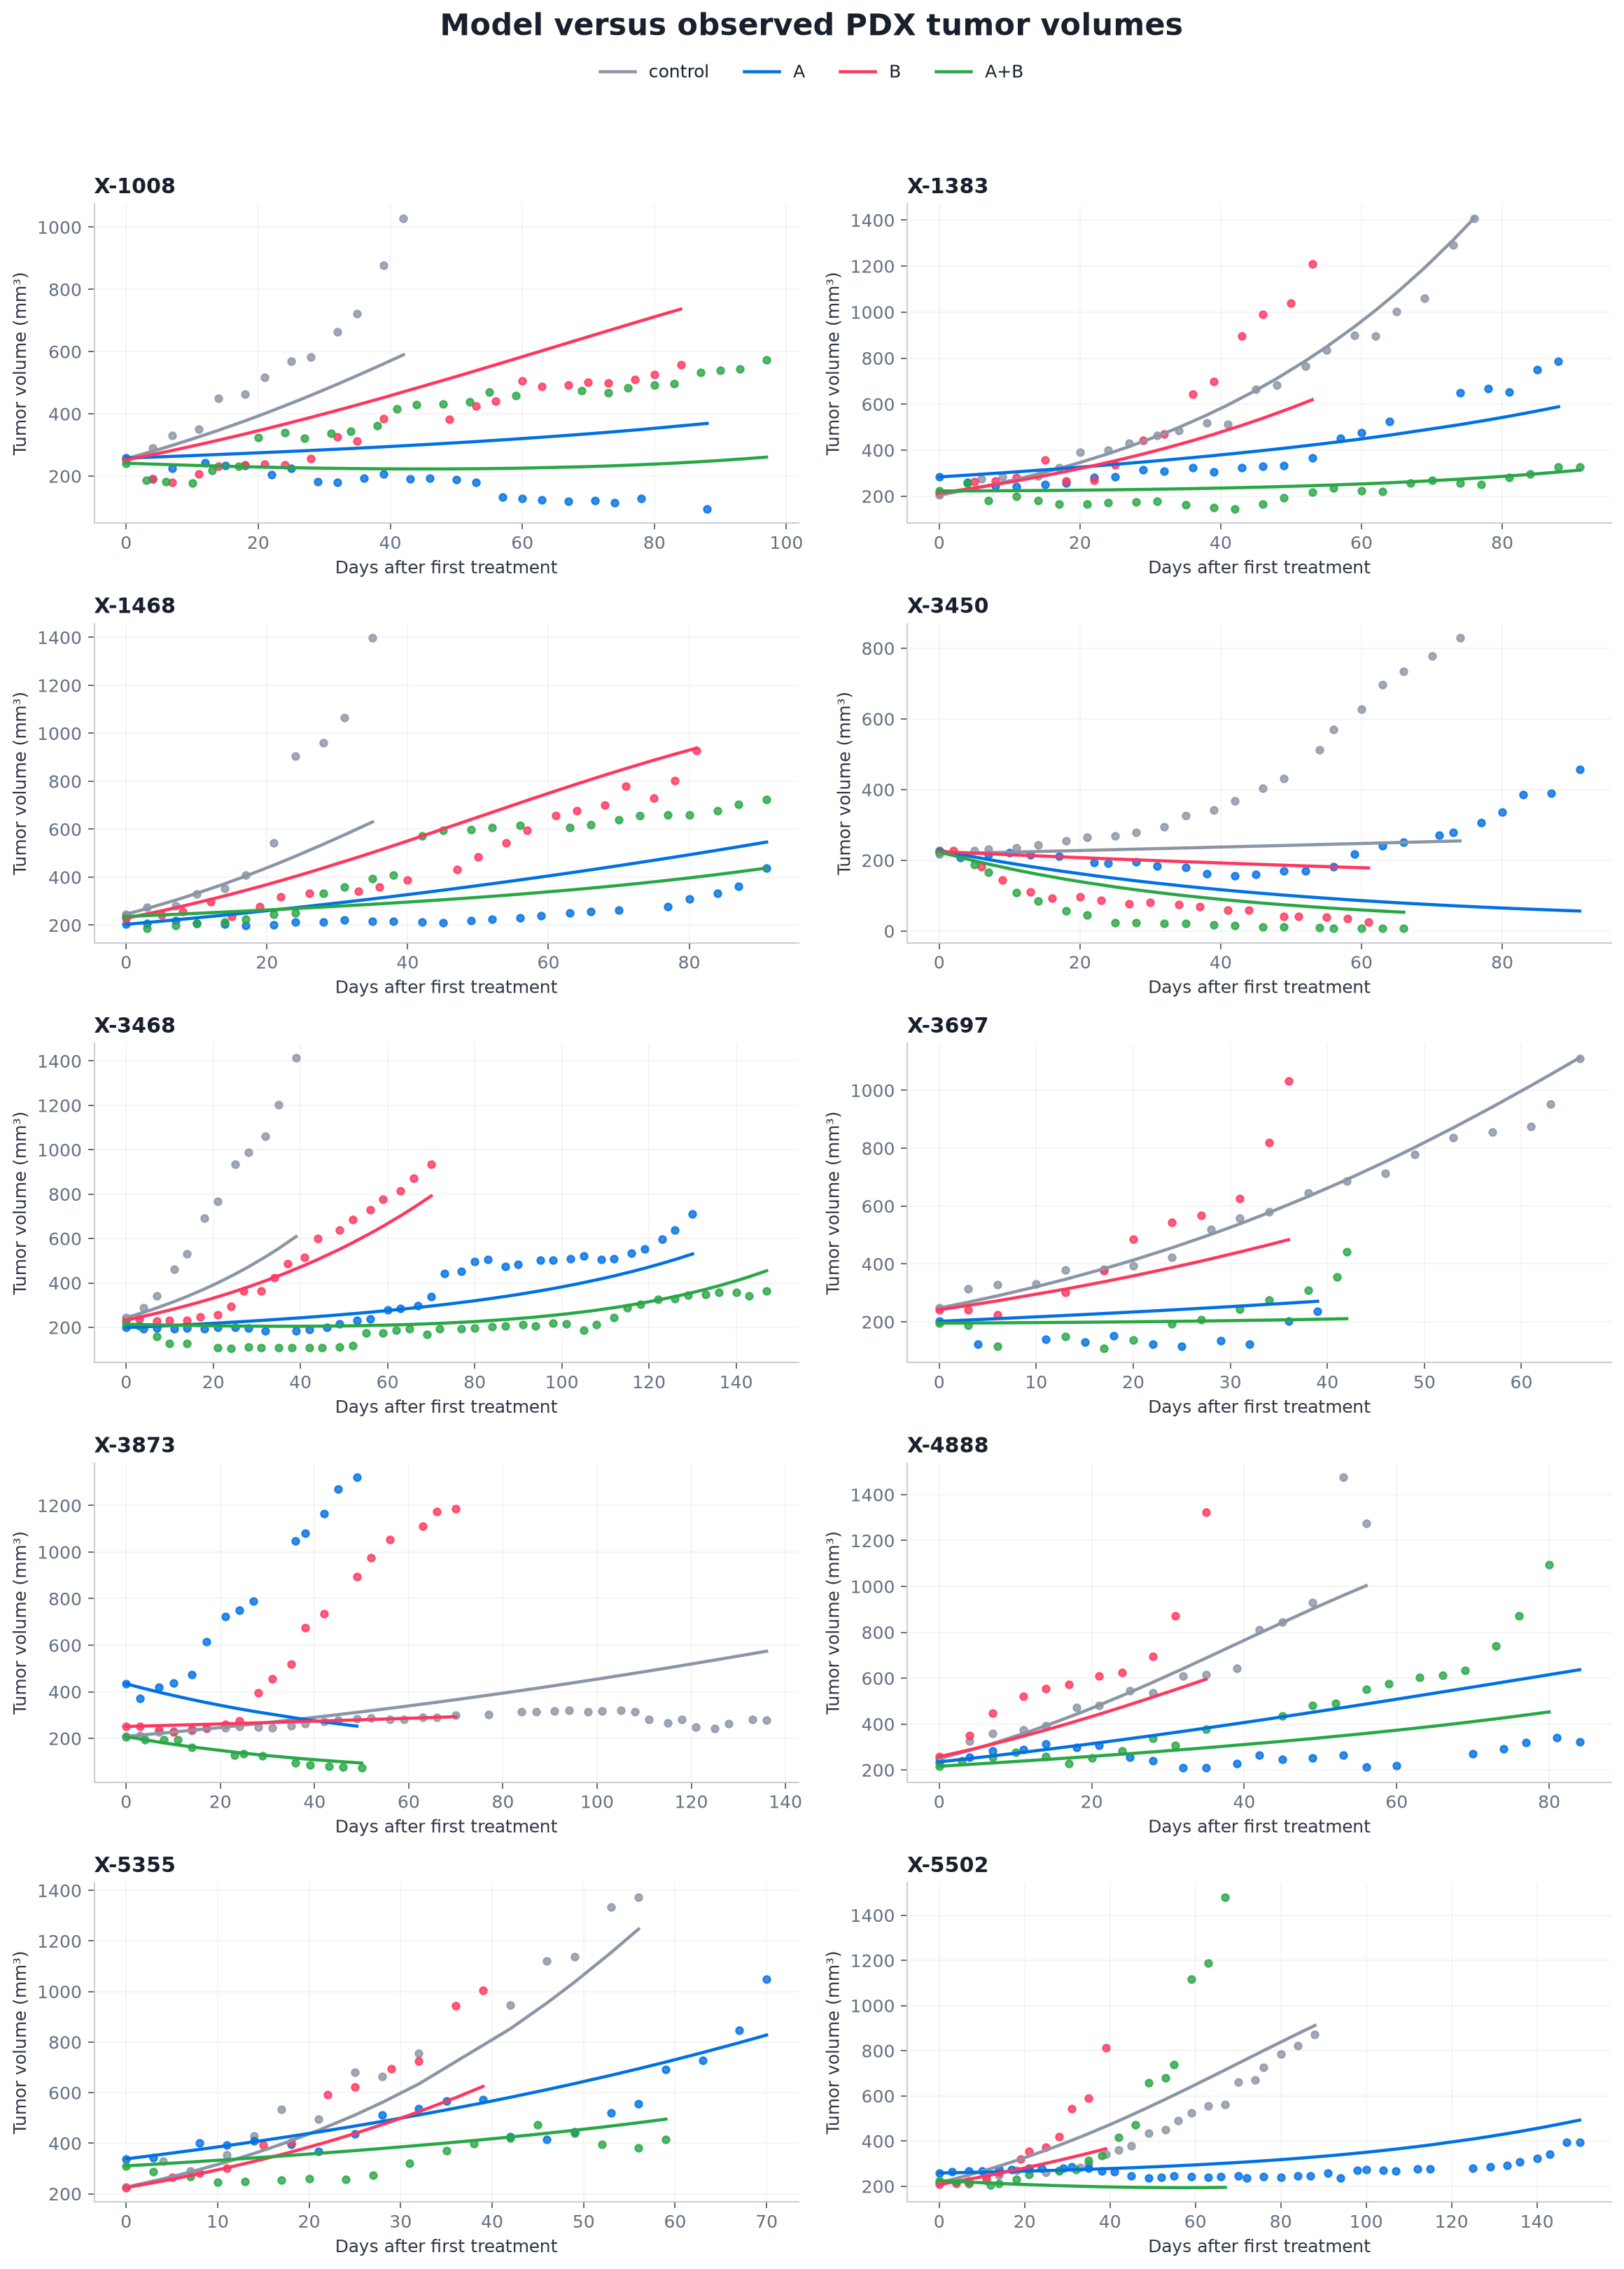
\includegraphics[height=.57\textheight]{../analysis/outputs/figures/model_vs_data.png}\caption{Observed tumor volumes (points) and fitted trajectories (lines) for each PDX line and arm. Colors are held fixed across report and site: control gray, BYL719 blue, LJM716 pink, combination green. Systematic mismatches remain, especially in some rapidly changing arms.}\end{figure}

\clearpage
\section*{Part D — Residuals and uncertainty}
\fig{residuals}{Residuals in log volume against time and fitted volume, with a normal quantile comparison. Curvature and outliers show that independent Gaussian error with a constant 0.15 log-scale spread is inadequate.}

\begin{center}\small\begin{tabular}{lrrrr}
\toprule Parameter & Estimate & Jacobian 95\% CI & 200 wild-bootstrap 95\% CI & Profile 95\% CI\\\midrule
$e_A$ & 0.0799 & [0.0641, 0.0957] & [0.0505, 0.1529] & see Fig. 3\\
$e_B$ & 0.0251 & [0.0092, 0.0410] & [0.0054, 0.0981] & see Fig. 3\\
$\psi$ & 26.73 & [$-3.33$, 56.79] & [$-1$, 50] & [10.62, 50]$^*$\\
\bottomrule\end{tabular}\end{center}
\vspace{-3pt}\noindent\footnotesize $^*$The profile upper endpoint reaches the fitted bound, so it is open rather than a finite upper confidence limit. The Jacobian interval extends beyond the bounds because it is a local linear approximation.\normalsize

The Jacobian covariance uses a residual-variance-scaled pseudoinverse of $J^TJ$. Our bootstrap resamples entire trajectory residual patterns by random sign flips, preserves measured baselines, and refits 200 times (200 completed). It retains serial patterns within a mouse, though with only one mouse per arm it cannot estimate between-mouse biological variation. The bootstrap interval touching both fit bounds and the local covariance interval crossing zero temper the small conditional LRT $p$-value. At least eight of ten $K_i$ values sit at fit bounds; this is a clear practical-identifiability warning.

\clearpage
\section*{Part E — Identifiability and sensitivity}
\fig{profile_likelihood}{Profile likelihood for $e_A$, $e_B$, and $\psi$. At each fixed grid value, all other parameters are optimized again; the horizontal threshold is the 95\% one-parameter $\chi^2$ cutoff. The broad $\psi$ profile reaches the upper parameter bound.}

\fig{parameter_correlation}{Correlation matrix inferred from the local fit Jacobian. Strong off-diagonal magnitudes reveal parameter compensation, particularly among growth, capacity, drug effects, and interaction. Boundary fits make this local matrix an imperfect global uncertainty summary.}

\clearpage
\section*{Part E — Local perturbations}
\fig{sensitivity_tornado}{Each fitted parameter is shifted by $\pm10\%$ while others remain at the optimum, subject to bounds. Bars summarize effects on weighted SSE and final combination volume; see exported \texttt{results.json} for numerical normalized coefficients. This is local sensitivity, not a refitted uncertainty interval.}

The profiles, bootstrap, and bound hits agree that response components can trade off under this design. A larger $\psi$ can offset small effective Emax occupancies; growth and capacity can compensate over a limited observation window. The positive likelihood profile conditional on the 0.6 dose ratio is therefore more restrictive than the structural uncertainty warrants. Neither volume-only data nor a single mouse per arm can identify the true exposure curve, resistant fraction, or a separate interaction for every PDX.

\section*{Part F — Biological interpretation}
The fitted mono-arm occupancies are $e_A=0.0799$ and $e_B=0.0251$. At the assumed combination dose, $e_{A,c}=0.0495$; Bliss predicts $E_{AB}=0.0734$, whereas the interaction fit predicts $0.1067$. At $\kappa=0.25$ day$^{-1}$, these imply mono kill rates of 0.0200/day and 0.00628/day and combination kill of 0.0267/day in sensitive volume. These are \emph{model rates}, not measured percentages of tumor shrinkage. Line-specific $r_i$ range from approximately 0.0025 to 0.0414/day (initial doubling times about 278 to 17 days); many $K_i$ estimates are boundary constrained, so line-level capacity biology should not be overinterpreted.

\clearpage
\section*{Part F — Interpretation, limitations, next experiment}
Under the reported differential BYL719 doses and proportional-exposure assumption, the fitted curves show apparent positive interaction. A full refit under equal effective BYL719 doses gives $\hat\psi=1.81$, likelihood-ratio $p=0.63$, $\Delta$AIC $=-1.77$, and $\Delta$BIC $=-6.50$ (Bliss favored). Thus the central conclusion depends on an exposure assumption that the source workbook cannot verify. The observed PDX cohort does not establish robust pharmacological synergy.

The original workbook has mutation/copy-number records. In the five relevant pathway genes, it annotates a PTEN deletion in X-1008, an AKT1 amplification and functional PIK3CA C420R mutation in X-3697, and an ERBB2 amplification in X-3873. These four records across ten lines do not support a credible genotype-response association; absence of an annotation is not wild type. The exact records are in \texttt{selected\_biomarkers.csv}. Mechanistically, inhibiting PI3K$\alpha$ while blocking HER3 feedback is plausible \cite{garrett,garner}; this rationale does not resolve the dose confounding.

The decisive limitations are the 1$\times$1$\times$1 design, no measured PK or intratumoral concentration, volume-only observations, fixed resistance kinetics, line-shared drug effects, large structured residuals, and bound-constrained carrying capacities. A stronger experiment would use multiple mice per arm, matched monotherapy and combination dose levels, serial drug concentrations and pathway readouts, and a priori interaction testing across dose pairs. Longitudinal lineage or resistant-cell measurements could separate true resistance from growth-rate and measurement artifacts.

\section*{Conclusions}
The data and an explicit ODE comparison yield a conditional interaction signal, but dose and model uncertainty prevent a reliable synergy claim. The project illustrates why a small $p$-value from a calibrated mechanistic model must be read alongside the experimental design, residuals, confidence intervals, and structural sensitivity.

\section*{Reproducibility and data availability}
\texttt{make all} downloads and verifies the official source workbook, builds the processed CSV, fits both models and uncertainty analyses, generates figures and this PDF, and exports the site JSON. Raw XLSX files are ignored because the source exceeds 50 MB; the processed CSV and fitting outputs are committed. The exact source file SHA-256 is stored in \texttt{selection.json}. Code, notebook, and figure exports are available at \url{https://github.com/zzkhxyz/endterm-bio}. The source paper DOI is \href{https://doi.org/10.1038/nm.3954}{10.1038/nm.3954}; the supplementary workbook has no separate DOI.

\vspace{-3pt}\begin{thebibliography}{9}\small
\bibitem{gao} Gao H et al. High-throughput screening using patient-derived tumor xenografts to predict clinical trial drug response. \emph{Nature Medicine}. 2015;21:1318--1325. \href{https://doi.org/10.1038/nm.3954}{doi:10.1038/nm.3954}.
\bibitem{baaz} Baaz M, Cardilin T, Jirstrand M. Analyzing the distribution of progression-free survival for combination therapies: a study of model-based translational predictive methods in oncology. \emph{European Journal of Pharmaceutical Sciences}. 2024;203:106901. \href{https://doi.org/10.1016/j.ejps.2024.106901}{doi:10.1016/j.ejps.2024.106901}.
\bibitem{garrett} Garrett JT et al. Combination of HER2 and PI3K inhibition in HER2-positive breast cancer models. \emph{PNAS}. 2013. \href{https://pmc.ncbi.nlm.nih.gov/articles/PMC3790862/}{PMC3790862}.
\bibitem{garner} Garner AP et al. An antibody that locks HER3 in the inactive conformation inhibits tumor growth. \emph{Cancer Research}. 2013. \href{https://pmc.ncbi.nlm.nih.gov/articles/PMC3924863/}{PMC3924863}.
\bibitem{euhus} Euhus DM et al. Tumor measurement in the nude mouse. \emph{Journal of Surgical Oncology}. 1986;31:229--234. \href{https://doi.org/10.1002/jso.2930310402}{doi:10.1002/jso.2930310402}.
\end{thebibliography}
\end{document}
